\documentclass{article}
\usepackage{authblk}

\usepackage{graphicx}% Include figure files
\usepackage{dcolumn}% Align table columns on decimal point
\usepackage{amsmath,amssymb}
\usepackage{bm}% bold math
\usepackage{enumitem}

\usepackage{hyperref}%to have clickable links
\hypersetup{
    colorlinks=true,
    linkcolor=blue,
    filecolor=magenta,      
    urlcolor=cyan,
}

\title{Multi-class classification on gene expression data}
\author[1]{Simone Daniotti}
\author[2]{Riccardo Castelli}

\affil[1]{Physics Department, University of Milan}
\affil[2]{Informatics Department, University of Milan}
\date{September 26, 2019}                     %% if you don't need date to appear
\setcounter{Maxaffil}{0}
\renewcommand\Affilfont{\itshape\small}

\begin{document}

  \maketitle
  
  
\begin{abstract}
Your abstract goes here...
...
\end{abstract}

\tableofcontents


\section{Dataset description}

The dataset for this work is taken from UCI Machine Learning Repo (available at \url{https://archive.ics.uci.edu/ml/datasets/gene+expression+cancer+RNA-Seq}) \cite{Dua:2019}; this is part of the RNA-Seq (HiSeq, a tool for measuring gene expression levels) PANCAN data set. It is a collection of gene expression levels of patients having different types of tumor: BRCA(breast), KIRC(kidney), COAD(colon), LUAD(lung) and PRAD(prostate).
These data represent the quantity of gene information used in the synthesis of a functional gene product. For further information, we refer to \cite{weinstein2013cancer}.


%%%%%%%%%%%%%%%%%%%%%%%%%%%%%%%%%%%%%%%%%%%%%%%

\section{Dataset Manipulation}


\subsection{Preliminary manipulation}
Both dataset and labels can be downloaded in a csv ('comma separated value') format, then can be easily imported in a Pandas Dataframe (\url{https://pandas.pydata.org/}). The first column represents patient's ID: it has been removed because it is useless for our purposes.



\subsection{Label handling}
The labels are strings representing the five types of cancer. Learning models can be created using raw features(in the case of trees and forests), using Label Encoding or One-hot Encoding.
Label Encoding creates a map between the string and an ordered sequence of natural numbers, from 0 to 4 in our case.
One-hot encoding creates a single binary label for each class, changing the task of the learning model to a multi-label problem.



\subsection{Train and Test Set}

For training the net and then evaluating it, we split the dataset in training and test set using the Sklearn library $train\_test\_split$ (\url{https://scikit-learn.org/stable/modules/generated/sklearn.model_selection.train_test_split.html}). We set the seed of the random split and the proportions between the two sets: test set is $0.15$ of the entire database.

\subsection{Class Weighting}


%%%%%%%%%%%%%%%%%%%%%%%%%%%%%%%%%%%%%%%%%%%%%%%


\section{Architectures}
There are lots of books reviewing these architectures and concepts. Here we refer to \cite{geron2017hands} , \cite{bishop2006pattern} \cite{hertz1991introduction}.

\subsection{Support Vector Machines (SVM)}

\subsection{Decision Tree Classifier and Random Forests}

Decision Trees are versatile Machine Learning algorithms that can perform both classification and regression tasks, and even multioutput tasks. They are particularly useful in treating with complex data, such as a dataset that can hardly be represented by a vector in a multi-dimensional space: this is not our case, but we think it is useful to approach our problem with more simple models and evaluating them before \textit{deeping} in more difficult models.
Tree Classifiers have the structure of an \textit{ordered and rooted tree}. It is \textit{ordered} because the children of any internal node are numbered consecutively, and \textit{rooted} because splitting starts from only one node.
From that node, the model is built following the attribute selection measure.
Attribute selection measure is a heuristic for selecting the splitting criterion that partition data into the best possible manner.

\begin{figure}[h!]
\centering
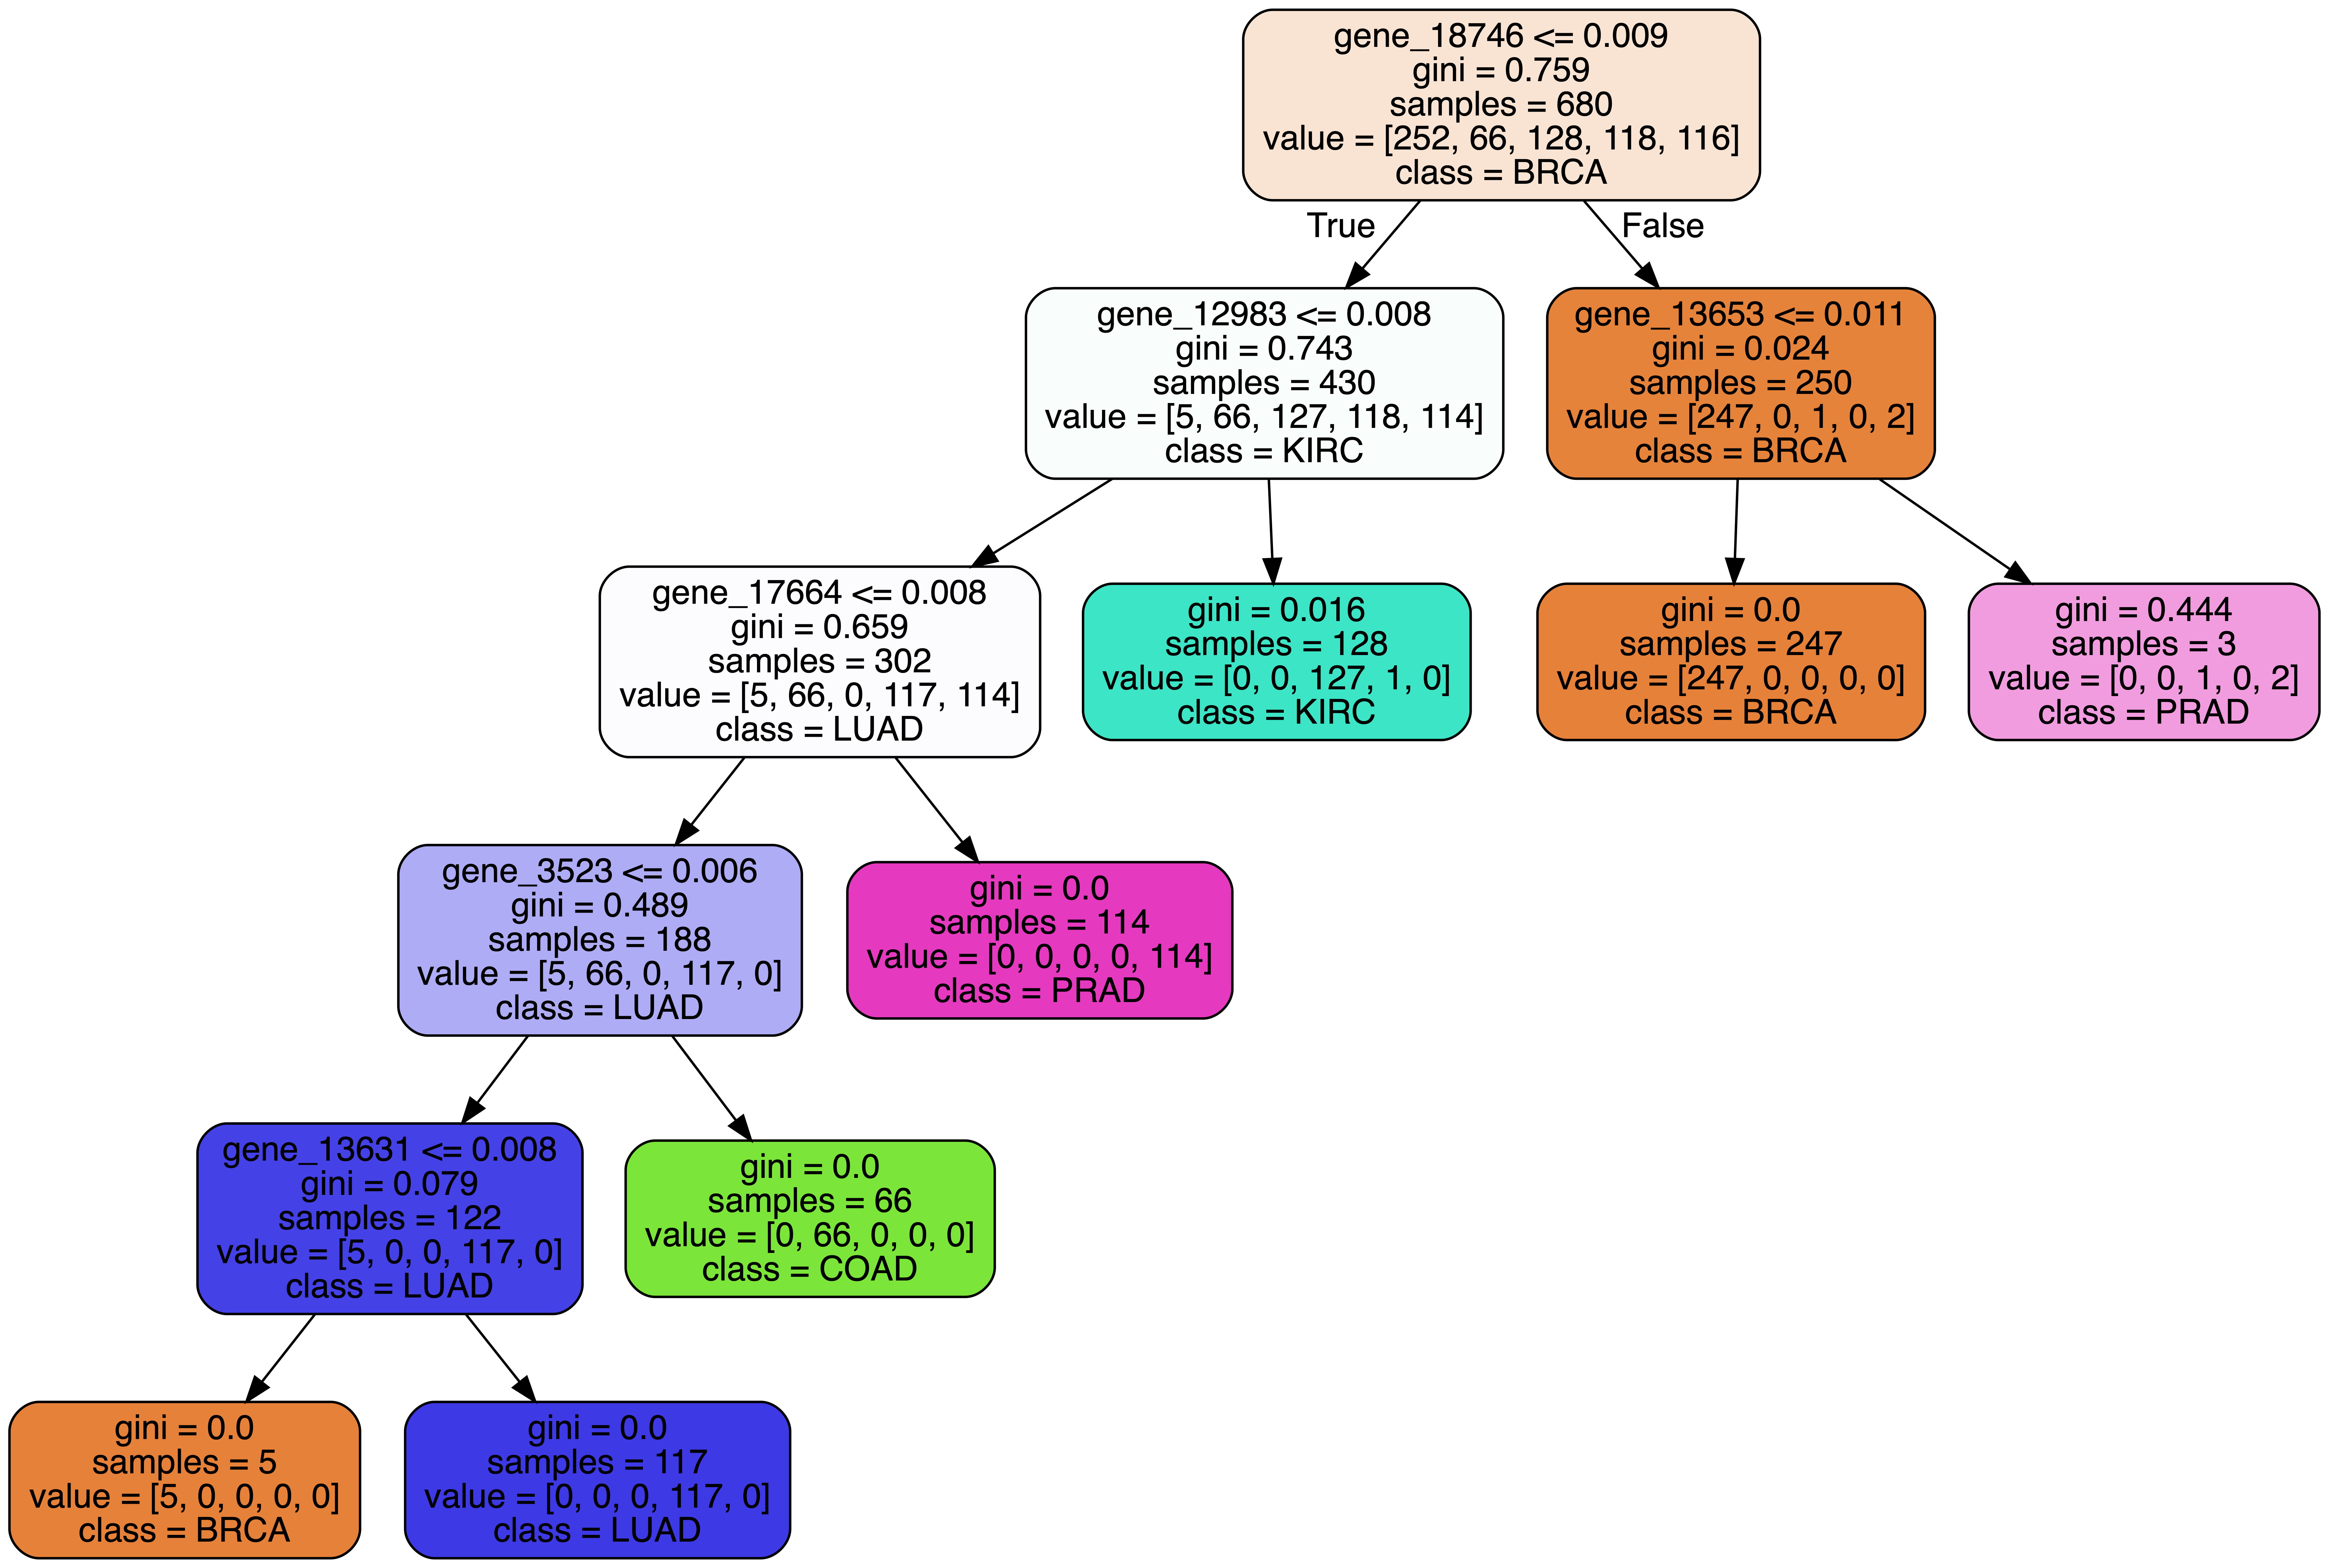
\includegraphics[width=\linewidth]{img/tree_best.png}
\caption{Shape of a tree classifier, with hyperparameters tuned by tecniques explained below.}
\label{fig1}
\end{figure}


Scikit-Learn uses the \textit{Classification And Regression Tree (CART) algorithm} to train Decision Trees.It works as follows: it first splits the training set in two subsets using a single feature k and a threshold $t_k$ . How does it choose $k$ and $t_k$? It searches for the pair $(k, t_k)$ that produces the purest subsets. The cost functions that the algorithm tries to minimize are different: most used are \textit{Gini Impurity} and \textit{Entropy}, tunable in Scikit-learn by the hyperparameter \textit{criterion}. Entropy hyperparameter measures Shannon's Entropy, a concept taken from information theory.
Each leaf of the tree corresponds to a possible classification label, so inserting datas of a patient from the root, the model $spits$ its classification. This can be a modality for building a predictor.


If you aggregate the predictions of a group of predictors (regulated by certain rules, such as majority rule..), you will often get better predictions than with the best individual predictor. A group of predictors is called an \textit{ensemble}; thus, this technique is called \textit{Ensemble Learning}, and an Ensemble Learning algorithm is called an \textit{Ensemble method}.
Training a group of Decision Tree Classifiers and gathering into one single predictor is called a \textit{Random Forest}.
The Random Forest algorithm introduces extra randomness when growing trees; instead of searching for the very best feature when splitting a node (as in the tree case), it searches for the best feature among a random subset of features. This results in a greater tree diversity.



\subsection{Deep Learning}

PARTE MANCANTE, DA FARE IN SEGUITO

\subsubsection{PyTorch}

PyTorch is a Python machine learning framework. It is built for creating learning algorithms based on graph models. 
It starts as a low-level library, but has a lot of high-level APIs for building big deep neural network in a bunch of code lines.
Its core element are Pytorch tensors, in the same way arrays are for Numpy, but are build to take advantage of GPU computing in an easy way.
Transition between low-level programming and APIs is truly continuous: this is a very important feature in building and tweaking a Deep Neural Network.
In depth, it has some useful built-in methods to handle training and evaluation, for example: autograd() to compute gradients and DataLoader() to handle training and batch loading.
All further documentation can be found here: \url{https://pytorch.org/}.

\subsubsection{Keras}

%%%%%%%%%%%%%%%%%%%%%%%%%%%%%%%%%%%%%%%%%%%%%%%


\section{Parameter optimization and Validation}

Once having built the net, a user must ensure that the model has a good generalizing capacity. Often, a too fitted net fails to predict in test set, in a sense longly described in the books cited above; this behaviour is called \textit{overfitting}.
In the sections below, we will review some of the tecniques used to avoid this feature and some characteristics of the models we studied.

\subsection{Cross-Validation}

One may desire a tecnique to evaluate generalization performances before testing the net. An idea could be to split again the training set, and using a part of it to test performances: this is called \textit{cross-validation}.
Scikit-Learn offers a great method to reach this task. Lets explain what is sklean's K-fold cross-validation: it randomly splits the training set into $k$ distinct subsets called \textit{folds}, then it trains and evaluates the model $k$ times, picking a different fold for evaluation every time and training on the other $k-1$ folds.

\subsection{Grid Search CV (and Random Search)}
Tweaking hyperparameters for each algorithm, one can see that some of them influence overfitting more than others: selecting the right parameters is a tedious job if one does it by hand.
Instead,one can use for example Scikit-Learn’s GridSearchCV. Passing to the function all values of some hyperparameters to evaluate, it will estimate all the possible combinations of them, using cross-validation. 

The grid search approach is fine when you are exploring relatively few combinations but when the hyperparameter search space is large, it is often preferable to use RandomizedSearchCV instead. This class is similar to grid search, but it evaluates random values for every parameter passed, taken from a probability distribution for each.
It is useful to explore larger parts of hyperparameter search space and to lighten computation.

Both functions were used, giving similar results in term of net performances.

\subsection{Architecture setting}
In general, but specially talking about deep neural networks, a user must define what parameters influence performances, how to evaluate net mistakes and how to improve model's predictions.

\subsubsection{Parameters}

\subsubsection{Losses}

Here we list some of the losses used during our work:

\begin{description}[align=left]

\item [Accuracy:] In multi-label and multi-class problems, this is a discrete measure of predictions, in the sense that results scores only when predition is exact (\url{https://scikit-learn.org/stable/modules/classes.html#module-sklearn.metrics});

\item [BCEWithLogitsLoss:] This loss combines a Sigmoid layer and the BCELoss in one single class. This version is more numerically stable than using a plain Sigmoid followed by a BCELoss as, by combining the operations into one layer, we take advantage of the log-sum-exp trick for numerical stability. The equation for the loss is:

\begin{equation}
loss(x,y) = \mathbb{E} \left[ \{ l_1,....,l_N\} ^\top \right] , 
\end{equation}
where
\begin{equation}
l_{n} = - w_{n} \left[ y_{n}  \log[\sigma(x_{n}) + (1-y_{n})  \log(1 - \sigma(x_{n})) \right]
\end{equation}


For further explanations and implementation, visit \url{https://pytorch.org/docs/stable/nn.html};

\item [CrossEntropyLoss:] This criterion combines nn.LogSoftmax() and nn.NLLLoss() in one single class. This criterion expects a class index in the range $[0,C-1]$ as the target for each value of a $1D$ tensor of size minibatch. The equation for the loss is the following:

\begin{equation}
loss(x,class) = - \log\left(\frac{exp(x[class])}{\sum_{j}{exp(x[j])}}\right)
\end{equation}

Documentation in the link above;

\item[LOSS DI KERAS]

\end{description}

\subsubsection{Optimizers}



%%%%%%%%%%%%%%%%%%%%%%%%%%%%%%%%%%%%%%%%

\section{Models Evaluation}

\subsection{PCA and Permutation Importance}

\subsection{Metrics}




%%%%%%%%%%%%%%%%%%%%%%%%%%%%%%%%
\section{Conclusions and Outlook}


%%%%%%%%%%%%%%%%%%%%%%%%%%%%%%%%%%%




%%%%%%%%%%%%%%%%%%%%%%%%%%%%%%%%%%%%%%%%%%

\bibliography{Bibliography}
\bibliographystyle{unsrt}


\end{document}